\Section{concurrent}{Concurrent Haskell}

Concurrent Haskell \cite{jones96concurrent} is an extension to Haskell
2010 \cite{haskell2010} adding support for explicitly threaded
concurrent programming.  The basic interface remains largely unchanged
in its current implementation, although a number of embellishments have
since been added, which we will cover in later sections:

\begin{itemize}
\item Asynchronous exceptions \cite{spj:asynch-exceptions} were added
  as a means for asynchronous cancellation of threads,
\item Software Transactional Memory was added \cite{stm}, allowing
  safe composition of concurrent abstractions, and making it possible
  to safely build larger concurrent systems.
\item The behaviour of Concurrent Haskell in the presence of calls to
  and from foreign languages was specified \cite{conc-ffi}
\end{itemize}

\Subsection{forking}{Forking Threads}

The basic requirement of concurrency is to be able to fork a new
thread of control.  In Concurrent Haskell this is achieved with the
@forkIO@ operation:

\begin{haskell}
forkIO :: IO () -> IO ThreadId
\end{haskell}

\noindent @forkIO@ takes a computation of type @IO ()@ as its
argument; that is, a computation in the @IO@ monad that eventually
delivers a value of type @()@.  The computation passed to @forkIO@ is
executed in a new \emph{thread} that runs concurrently with the other
threads in the system.  If the thread has effects, those effects will
be interleaved in an indeterminate fashion with the effects from other
threads.

To illustrate the interleaving of effects, let's try a simple example
in which two threads are created, once which continually prints the
letter @A@ and the other printing @B@\footnote{this is sample @fork.hs@}:

\begin{numhaskell}
import Control.Concurrent
import Control.Monad
import System.IO

main = do
  hSetBuffering stdout NoBuffering
  forkIO (forever (putChar 'A'))
  forkIO (forever (putChar 'B'))
  threadDelay (10^6)
\end{numhaskell}

\noindent Line 6 puts the output @Handle@ into non-buffered mode, so
that we can see the interleaving more clearly.  Lines 7 and 8 create
the two threads, and line 9 tells the main thread to wait for one
second (@10^6@ microseconds) and then exit.

When run, this program produces output something like this:

\begin{verbatim}
AAAAAAAAABABABABABABABABABABABABABABABABABABABABABABAB
ABABABABABABABABABABABABABABABABABABABABABABABABABABAB
ABABABABABABABABABABABABABABABABABABABABABABABABABABAB
ABABABABABABABABABABABABABABABABABABABABABABABABABABAB
\end{verbatim}

\noindent Note that the interleaving is non-deterministic: sometimes we get
strings of a single letter, but often the output switches regularly
between the two threads.  Why does it switch so regularly, and why
does each thread only get a chance to output a single letter before
switching?  The threads in this example are contending for a single
resource: the @stdout@ Handle, so scheduling is affected by how
contention for this resource is handled.  In the case of GHC a Handle
is protected by a lock implemented as an @MVar@ (described in the next
section).  We shall see shortly how the implementation of @MVar@s
causes the @ABABABA@ behaviour.

% ToDo: move this into a separate section and expand.

We emphasised earlier that concurrency is a program structuring
technique, or an abstraction.  Abstractions are practical when they
are efficient, and this is where GHC's implementation of threads comes
into its own.  Threads are extremely lightweight in GHC: a thread
typically costs less than a hundred bytes plus the space for its
stack, so the runtime can support literally millions of them, limited
only by the available memory.  Unlike OS threads, the memory used by
Haskell threads is movable, so the garbage collector can pack threads
together tightly in memory and eliminate fragmentation.  Threads can
also expand and shrink on demand, according to the stack demands of
the program.  When using multiple processors, the GHC runtime system
automatically migrates threads between cores in order to balance the
load.

User-space threading is not unique to Haskell, indeed many other
languages, including early Java implementations, have had support for
user-space threads (sometimes called ``green threads'').  It is often
thought that user-space threading hinders interoperability with
foreign code and libraries that are using OS threads, and this is one
reason that OS threads tend to be preferred.  However, with some
careful design it is possible to overcome these difficulties too, as
we shall see in \secref{conc-ffi}.

\Subsection{mvars}{Communication: MVars}

The lowest-level communication abstraction in Concurrent Haskell is
the @MVar@, whose interface is given below:

\begin{haskell}
data MVar a  -- abstract

newEmptyMVar :: IO (MVar a)
newMVar      :: a -> IO (MVar a)
takeMVar     :: MVar a -> IO a
putMVar      :: MVar a -> a -> IO ()
\end{haskell}

\noindent An @MVar@ can be thought of as a box that is either empty
or full. The @newEmptyMVar@ operation creates a new empty box, and @newMVar@ creates
a new full box containing the value passed as its argument.  The @putMVar@
operation puts a value into the box, but blocks (waits) if the box is
already full.  Symmetrically, the @takeMVar@ operation removes the value
from a full box but blocks if the box is empty.

@MVar@s generalise several simple concurrency abstractions:

\begin{itemize}
\item @MVar ()@ is a \emph{lock}; @takeMVar@ acquires the lock and
  @putMVar@ releases it again.\footnote{It works perfectly well the
    other way around too, just be sure to be consistent about the policy.}  An @MVar@ used in this way can protect
  shared mutable state or critical sections.

\item An @MVar@ is a one-place channel, which can be used for
  asynchronous communication between two threads.  In
  \secref{channels} we show how to build unbounded buffered channels
  from @MVar@s.

\item An @MVar@ is a useful container for shared mutable state.  For
  example, a common design pattern in Concurrent Haskell when several
  threads need read and write access to some state, is to represent
  the state value as an ordinary immutable Haskell data structure
  stored in an @MVar@.  Modifying the state consists of taking the
  current value with @takeMVar@ (which implicitly acquires a lock),
  and then placing a new value back in the @MVar@ with @putMVar@
  (which implicitly releases the lock again).

% ToDo:
% We'll come back to shared mutable state in \secref{conc-data}.
\end{itemize}

We can also use @MVar@s to do some simple asynchronous I/O.  Suppose
we want to download some web pages concurrently and wait for them all
to download before continuing.  We are given the following function to
download a web page:

\begin{haskell}
getURL :: String -> IO ByteString
\end{haskell}

\noindent Let's use this to download two URLs concurrently:

\begin{numhaskell}
do
   m1 <- newEmptyMVar
   m2 <- newEmptyMVar

   forkIO $ do
     r <- getURL "http://www.wikipedia.org/wiki/Shovel"
     putMVar m1 r

   forkIO $ do
     r <- getURL "http://www.wikipedia.org/wiki/Spade"
     putMVar m2 r

   r1 <- takeMVar m1
   r2 <- takeMVar m2
   return (r1,r2)
\end{numhaskell}

\noindent Lines 2--3 create two new empty @MVar@s to hold the
results.  Lines 5--7 fork a new thread to download the first URL; when
the download is complete the result is placed in the @MVar@ @m1@, and
lines 9--11 do the same for the second URL, placing the result in @m2@.
In the main thread, line 13 waits for the result from @m1@, and line 14
waits for the result from @m2@ (we could do these in either order), and
finally both results are returned.

This code is rather verbose.  We could shorten it by using various
existing higher-order combinators from the Haskell library, but a
better approach would be to extract the common pattern as a new
abstraction: we want a way to perform an action \emph{asynchronously},
and later wait for its result.  So let's define an interface that does
that, using @forkIO@ and @MVar@s:

\begin{numhaskell}
newtype Async a = Async (MVar a)

async :: IO a -> IO (Async a)
async io = do
  m <- newEmptyMVar
  forkIO $ do r <- io; putMVar m r
  return (Async m)

wait :: Async a -> IO a
wait (Async m) = readMVar m
\end{numhaskell}

\noindent Line 1 defines a datatype @Async@ that represents an
asynchronous action that has been started.  Its implementation is just
an @MVar@ that will contain the result; creating a new type here might
seem like overkill, but later on we will extend the @Async@ type to
support more operations, such as cancellation.

The @wait@ operation uses @readMVar@, defined
thus\footnote{@readMVar@ is a standard operation provided by
  the @Control.Concurrent@ module}:

\begin{haskell}
readMVar :: MVar a -> IO a
readMVar m = do
  a <- takeMVar m
  putMVar m a
  return a
\end{haskell}

\noindent that is, it puts back the value into the @MVar@ after
reading it, the point being that we might want to call @wait@ multiple
times, or from different threads.

Now, we can use the @Async@ interface to clean up our
web-page downloading example:

\begin{numhaskell}
do
   a1 <- async $ getURL "http://www.wikipedia.org/wiki/Shovel"
   a2 <- async $ getURL "http://www.wikipedia.org/wiki/Spade"
   r1 <- wait a1
   r2 <- wait a2
   return (r1,r2)
\end{numhaskell}

Much nicer!  To demonstrate this working, we can make a small wrapper
that downloads a URL and reports how much data was downloaded and how
long it took\footnote{the full code can be found in the sample @geturls.hs@}:

\begin{haskell}
sites = ["http://www.google.com",
         "http://www.bing.com",
         ... ]

main = mapM (async.http) sites >>= mapM wait
 where
   http url = do
     (page, time) <- timeit $ getURL url
     printf "downloaded: %s (%d bytes, %.2fs)\n"
        url (B.length page) time
\end{haskell}

\noindent which results in something like this:

{\scriptsize
\begin{verbatim}
downloaded: http://www.google.com (14524 bytes, 0.17s)
downloaded: http://www.bing.com (24740 bytes, 0.18s)
downloaded: http://www.wikipedia.com/wiki/Spade (62586 bytes, 0.60s)
downloaded: http://www.wikipedia.com/wiki/Shovel (68897 bytes, 0.60s)
downloaded: http://www.yahoo.com (153065 bytes, 1.11s)
\end{verbatim}
}

\begin{figure}
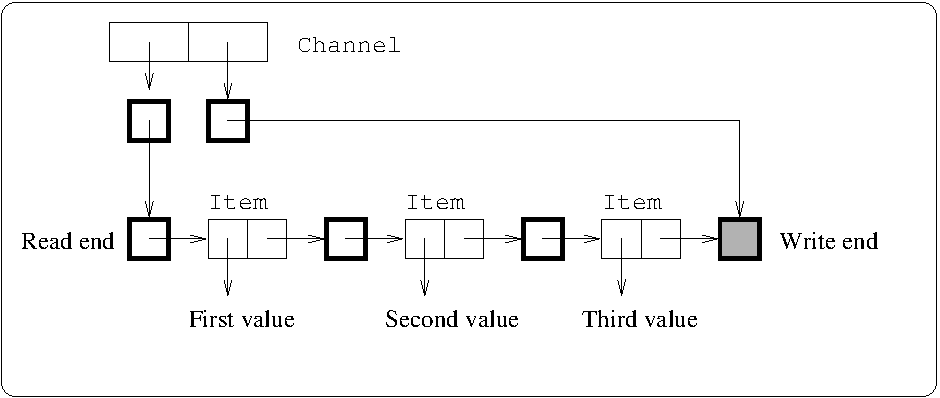
\includegraphics[scale=0.8]{channel.pdf}
\label{fig:channels}
\caption{Structure of the buffered channel implementation}
\end{figure}

\Subsubsection{channels}{Channels}

One of the strengths of @MVar@s is that they are a useful building
block out of which larger abstractions can be constructed.  Here we
will use @MVar@s to construct a unbounded buffered channel, supporting
the following basic interface:

\begin{haskell}
data Chan a

newChan   :: IO (Chan a)
readChan  :: Chan a -> IO a
writeChan :: Chan a -> a -> IO ()
\end{haskell}

\noindent This channel implementation first appeared in
\citet{jones96concurrent} (although the names were slightly
different), and is available in the Haskell module
@Control.Concurrent.Chan@.  The structure of the implementation is
represented diagrammatically in \figref{channels}, where each bold box
represents an @MVar@ and the lighter boxes are ordinary Haskell data
structures.  The current contents of the channel are represented as a
@Stream@, defined like this:

\begin{haskell}
type Stream a = MVar (Item a)
data Item a   = Item a (Stream a)
\end{haskell}

\noindent The end of the stream is represented by an empty @MVar@,
which we call the ``hole'', because it will be filled in when a new
element is added.  The channel itself is a pair of @MVar@s, one
pointing to the first element of the @Stream@ (the read position), and
the other pointing to the empty @MVar@ at the end (the write
position):

\begin{haskell}
data Chan a
 = Chan (MVar (Stream a))
        (MVar (Stream a))
\end{haskell}

To construct a new channel we must first create an empty @Stream@, which
is just a single empty @MVar@, and then the @Chan@ constructor with
@MVar@s for the read and write ends, both pointing to the empty
@Stream@:

\begin{haskell}
newChan :: IO (Chan a)
newChan = do
   hole  <- newEmptyMVar
   readVar  <- newMVar hole
   writeVar <- newMVar hole
   return (Chan readVar writeVar)
\end{haskell}

To add a new element to the channel we must make an @Item@ with a new
hole, fill in the current hole to point to the new item, and adjust
the write-end of the @Chan@ to point to the new hole:

\begin{haskell}
writeChan :: Chan a -> a -> IO ()
writeChan (Chan _ writeVar) val = do
  new_hole <- newEmptyMVar
  old_hole <- takeMVar writeVar
  putMVar writeVar new_hole
  putMVar old_hole (Item val new_hole)
\end{haskell}

To remove a value from the channel, we must follow the read end of the
@Chan@ to the first @MVar@ of the stream, take that @MVar@ to get the
@Item@, adjust the read end to point to the next @MVar@ in the stream,
and finally return the value stored in the @Item@:

\begin{numhaskell}
readChan :: Chan a -> IO a
readChan (Chan readVar _) = do
  stream <- takeMVar readVar
  Item val new <- takeMVar stream
  putMVar readVar new
  return val
\end{numhaskell}

\noindent Consider what happens if the channel is empty.  The first
@takeMVar@ (line 3) will succeed, but the second @takeMVar@ (line 4)
will find an empty hole, and so will block.  When another thread calls
@writeChan@, it will fill the hole, allowing the first thread to
complete its @takeMVar@, update the read end (line 5) and finally
return.

If multiple threads concurrently call @readChan@, the first one will
successfully call @takeMVar@ on the read end, but the subsequent
threads will all block at this point until the first thread completes
the operation and updates the read end.  If multiple threads call
@writeChan@, a similar thing happens: the write end of the @Chan@ is
the synchronisation point, only allowing one thread at a time to add
an item to the channel.  However, the read and write ends being
separate @MVar@s allows concurrent @readChan@ and @writeChan@
operations to proceed without interference.

This implementation allows a nice generalisation to \emph{multicast}
channels without changing the underlying structure.  The idea is to
add one more operation:

\begin{haskell}
dupChan :: Chan a -> IO (Chan a)
\end{haskell}

\noindent which creates a duplicate @Chan@ with the following
semantics:

\begin{itemize}
\item The new @Chan@ begins empty,
\item Subsequent writes to either @Chan@ are read from both; that is,
  reading an item from one @Chan@ does not remove it from the other.
\end{itemize}

The implementation is straightforward:

\begin{haskell}
dupChan :: Chan a -> IO (Chan a)
dupChan (Chan _ writeVar) = do
   hole       <- takeMVar writeVar
   putMVar writeVar hole
   newReadVar <- newMVar hole
   return (Chan newReadVar writeVar)
\end{haskell}

\noindent Both channels share a single write-end, but they have
independent read-ends.  The read end of the new channel is initialised
to point to the hole at the end of the current contents.

Sadly, this implementation of @dupChan@ does not work!  Can you see
the problem?  The definition of @dupChan@ itself is not at fault, but
combined with the definition of @readChan@ given earlier it does not
implement the required semantics.  The problem is that @readChan@ does
not replace the contents of a hole after having read it, so if
@readChan@ is called to read values from both the channel returned by
@dupChan@ and the original channel, the second call will block.  The fix is to change a
@takeMVar@ to @readMVar@ in the implementation of @readChan@:

\begin{numhaskell}
readChan :: Chan a -> IO a
readChan (Chan readVar _) = do
  stream <- takeMVar readVar
  Item val new <- readMVar stream -- modified
  putMVar readVar new
  return val
\end{numhaskell}

\noindent Line 4 returns the @Item@ back to the @Stream@, where it can
be read by any duplicate channels created by @dupChan@.

Before we leave the topic of channels, consider one more extension to
the interface that was described as an ``easy extension'' and left as
an exercise by \citet{jones96concurrent}:

\begin{haskell}
unGetChan :: Chan a -> a -> IO ()
\end{haskell}

\noindent the operation @unGetChan@ pushes a value back on the read
end of the channel.  Leaving aside for a moment the fact that the
interface does not allow the atomic combination of @readChan@ and
@unGetChan@ (which would appear to be an important use case), let us
consider how to implement @unGetChan@.  The straightforward
implementation is as follows:

\begin{numhaskell}
unGetChan :: Chan a -> a -> IO ()
unGetChan (Chan readVar _) val = do
   new_read_end <- newEmptyMVar
   read_end <- takeMVar readVar
   putMVar new_read_end (Item val read_end)
   putMVar readVar new_read_end
\end{numhaskell}

\noindent we create a new hole to place at the front of the @Stream@
(line 3), take the current read end (line 4) giving us the current
front of the stream, place a new @Item@ in the new hole (line 5), and
finally replace the read end with a pointer to our new item.

Simple testing will confirm that the implementation works.  However,
consider what happens when the channel is empty, there is already a
blocked @readChan@, and another thread calls @unGetChan@.  The desired
semantics is that @unGetChan@ succeeds, and @readChan@ should return
with the new element.  What actually happens in this case is deadlock:
the thread blocked in @readChan@ will be holding the read-end @MVar@,
and so @unGetChan@ will also block (line 4) trying to take the read
end.  As far as we know, there is no implementation of @unGetChan@
that has the desired semantics.

The lesson here is that programming larger structures with @MVar@ can
be much trickier than it appears.  As we shall see shortly, life gets
even more difficult when we consider exceptions.  Fortunately there is
a solution, that we will describe in \secref{stm}.

Despite the difficulties with scaling @MVar@s up to larger
abstractions, @MVar@s do have some nice properties, as we shall see in
the next section.

\Subsubsection{fairness}{Fairness}

Fairness is a well-studied and highly technical subject, which we do
not attempt to review here.  Nevertheless, we wish to highlight one
particularly important guarantee provided by @MVar@s with respect to
fairness:

\begin{quote}
No thread can be blocked indefinitely on an @MVar@ unless another
thread holds that @MVar@ indefinitely.
\end{quote}

In other words, if a thread $T$ is blocked in @takeMVar@, and there
are regular @putMVar@ operations on the same @MVar@, then it is
guaranteed that at some point thread $T$'s @takeMVar@ will return.  In
GHC this guarantee is implemented by keeping blocked threads in a FIFO
queue attached to the @MVar@, so eventually every thread in the queue
will get to complete its operation as long as there are other threads
performing regular @putMVar@ operations (an equivalent guarantee
applies to threads blocked in @putMVar@ when there are regular
@takeMVar@s).  Note that it is not enough to merely \emph{wake up} the
blocked thread, because another thread might run first and take
(respectively put) the @MVar@, causing the newly woken thread to go to
the back of the queue again, which would invalidate the fairness
guarantee.  The implementation must therefore atomically wake up the
blocked thread \emph{and} perform the blocked operation, which is
exactly what GHC does.

\paragraph{Fairness in practice}  Recall our example from \secref{forking}, where we had two threads,
one printing @A@s and the other printing @B@s, and the output was
often perfect alternation between the two: @ABABABABABABABAB@.  This
is an example of the fairness guarantee in practice.  The @stdout@
handle is represented by an @MVar@, so when both threads attempt to
call @takeMVar@ to operate on the handle, one of them wins and the
other becomes blocked.  When the winning thread completes its
operation and calls @putMVar@, the scheduler wakes up the blocked
thread \emph{and} completes its blocked @takeMVar@, so the original
winning thread will immediately block when it tries to re-acquire the
handle.  Hence this leads to perfect alternation between the two
threads.  The only way that the alternation pattern can be broken is if one
thread is pre-empted while it is not holding the @MVar@; indeed this
does happen from time to time, as we see the occasional long string of
a single letter in the output.

%  that this implementation does rely on some fairness in the
% scheduler too: the thread waiting to do the next @putMVar@ must not be
% indefinitely delayed, otherwise the fairness guarantee on @MVar@s
% fails.  At the current time GHC is using round-robin scheduling which
% satisfies this property.

A consequence of the fairness implementation is that, when multiple
threads are blocked, \emph{we only need to wake up a single thread}.
This single wakeup property is a particularly important performance
characteristic when a large number of threads are contending for a
single @MVar@.  As we shall see later, it is the fairness guarantee
together with the single-wakeup property which means that @MVar@s are
not completely subsumed by Software Transactional Memory.

\Subsection{async-exceptions}{Cancellation: Asynchronous Exceptions}

In an interactive application, it is often important for one thread to
be able to \emph{interrupt} the execution of another thread when some
particular condition occurs.  Some examples of this kind of behaviour
in practice include:

\begin{itemize}
\item In a web browser, the thread downloading the web page and the
  thread rendering the page need to be interrupted when the user
  presses the ``stop'' button.

\item A server application typically wants to give a client a set
  amount of time to issue a request before closing its connection, so
  as to avoid dormant connections using up resources.

\item An application in which a compute-intensive thread is working
  (say, rendering a visualisation of some data), and the input data
  changes due to some user input.
\end{itemize}

The crucial design decision in supporting cancellation is whether the
intended victim should have to poll for the cancellation condition,
or whether the thread is immediately cancelled in some way.  This is a
tradeoff:

\begin{enumerate}
\item If the thread has to poll, there is a danger that the programmer
  may forget to poll regularly enough, and the thread will become
  unresponsive, perhaps permanently so.  Unresponsive threads lead to
  hangs and deadlocks, which are particularly unpleasant from a
  user's perspective.
\item If cancellation happens asynchronously, critical sections that
  modify state need to be protected from cancellation, otherwise
  cancellation may occur mid-update leaving some data in an
  inconsistent state.
\end{enumerate}

In fact, the choice is really between doing only (1), or doing both
(1) and (2), because if (2) is the default, protecting a critical
section amounts to switching to polling behaviour for the duration of
the critical section.

In most imperative languages it is unthinkable for (2) to be the
default, because so much code is state-modifying.  Haskell has a
distinct advantage in this area, however: most code is purely
functional, so it can be safely aborted or suspended, and later
resumed, without affecting correctness.  Moreover our hand is
forced: purely functional code cannot by definition poll for the
cancellation condition, so it must be cancellable by default.

Therefore, fully-asynchronous cancellation is the only sensible
default in Haskell, and the design problem reduces to deciding how
cancellation appears to code in the @IO@ monad.

It makes sense for cancellation to behave like an exception, since
exceptions are already a fact of life in the @IO@ monad, and the usual
idioms for writing @IO@ monad code include exception handlers to
release resources and clean up in the event of an error.  For example,
to perform an operation that requires a temporary file, we would use
the @bracket@ combinator to ensure that the temporary file is always
removed, even if the operation raises an exception:

\begin{haskell}
  bracket (newTempFile "temp")
          (\file -> removeFile file)
          (\file -> ...)
\end{haskell}

\noindent where @bracket@ is defined thus:

\begin{haskell}
bracket :: IO a -> (a -> IO b) -> (a -> IO c) -> IO c
bracket before after during = do
  a <- before
  c <- during a `onException` after a
  after a
  return c
\end{haskell}

\noindent and @onException@ executes its first argument, and if an
exception is thrown, executes its second argument before re-throwing
the exception.

\begin{haskell}
onException :: IO a -> IO b -> IO a
\end{haskell}

We want exception handlers to run in the event of cancellation, so
cancellation should be an exception.  However, there's a fundamental
difference between the kind of exception thrown by @openFile@ when the
file does not exist, for example, and an exception that may arise
\emph{at any time} because the user pressed the ``stop'' button.  We
call the latter kind an \emph{asynchronous} exception, for obvious
reasons.  (We do not review the Haskell support for \emph{synchronous}
exceptions here; for that see the Haskell 2010 report
\cite{haskell2010} and the documentation for the @Control.Exception@
module).

To initiate an asynchronous exception, Haskell provides the @throwTo@
primitive which throws an exception from one thread to
another \cite{spj:asynch-exceptions}:

\begin{haskell}
throwTo :: Exception e => ThreadId -> e -> IO ()
\end{haskell}

\noindent the @Exception@ constraint requires that the exception value
being thrown is an instance of the @Exception@ class, which implements
a simple hierarchy \cite{extensible-exceptions}.  The @ThreadId@ is a
value previously returned by @forkIO@, and may refer to a thread in
any state: running, blocked, or finished (in the latter case,
@throwTo@ is a no-op).

To illustrate the use of @throwTo@, we now elaborate the earlier
example in which we downloaded several web pages concurrently, to
allow the user to hit @'q'@ at any time to stop the downloads.

First, we will extend our @Async@ mini-API to allow cancellation.  We
add one operation:

\begin{haskell}
cancel :: Async a -> IO ()
\end{haskell}

\noindent which cancels an existing @Async@.  If the operation has
already completed, @cancel@ has no effect.  The @wait@ operation
cannot just return the result of the @Async@ any more, since it may
have been cancelled.  Therefore, we extend @wait@ to return
@Either SomeException a@, containing either the exception raised during the
operation, or its result:

\begin{haskell}
wait :: Async a -> IO (Either SomeException a)
\end{haskell}

\noindent (@SomeException@ is the root of the exception hierarchy in Haskell.)
In order to implement the new interface, we need to extend the @Async@
type to include the @ThreadId@ of the child thread, and the @MVar@
holding the result must now hold @Either SomeException a@.

\begin{haskell}
data Async a = Async ThreadId (MVar (Either SomeException a))
\end{haskell}

\noindent Given this, the implementation of @cancel@ just throws an
exception to the thread:

\begin{haskell}
cancel :: Async a -> IO ()
cancel (Async t var) = throwTo t ThreadKilled
\end{haskell}

\noindent (@ThreadKilled@ is an exception provided by the Haskell exception
library and is typically used for cancelling threads in this way.)
The implementation of @wait@ is trivial.
The remaining piece of the implementation is the @async@ operation,
which must now include an exception handler to catch the exception and
store it in the @MVar@:

\begin{haskell}
async :: IO a -> IO (Async a)
async io = do
   m <- newEmptyMVar
   t <- forkIO $ (do r <- io; putMVar m (Right r))
                   `catch` \e -> putMVar m (Left e)
   return (Async t m)
\end{haskell}

Now, we can change the @main@ function of the example to support
cancelling the downloads:

\begin{numhaskell}
main = do
  as <- mapM (async.http) sites

  forkIO $ do
     hSetBuffering stdin NoBuffering
     forever $ do
        c <- getChar
        when (c == 'q') $ mapM_ cancel as

  rs <- mapM wait as
  printf "%d/%d finished\n" (length (rights rs)) (length rs)
\end{numhaskell}

\noindent Line 2 starts the downloads as before.  Lines 4--8 fork a
new thread that repeatedly reads characters from the standard input,
and if a @q@ is found, calls @cancel@ on all the @Async@s.  Line 10
waits for all the results (complete or cancelled), and line 11 emits a
summary with a count of how many of the operations completed without
being cancelled.  If we run the sample\footnote{full code is in the
  sample @geturlscancel.hs@} and hit @`q`@ fast enough, we see
something like this:

\begin{verbatim}
downloaded: http://www.google.com (14538 bytes, 0.17s)
downloaded: http://www.bing.com (24740 bytes, 0.22s)
q2/5 finished
\end{verbatim}

Note that this works even though the program is sitting atop a large
and complicated HTTP library that provides no direct support for
either cancellation or asynchronous I/O.  Haskell's support for
cancellation is modular in this respect: most library code needs to do
nothing to support it, although there are some simple and unintrusive
rules that need to be followed when dealing with state, as we shall
see in the next section.

\Subsubsection{mask}{Masking asynchronous exceptions}

As we mentioned earlier, the danger with fully asynchronous exceptions
is that one might fire while we are in the middle of updating some
shared state, leaving the data in an inconsistent state, and with a
high probability leading to mayhem later.

Hence, we certainly need a way to control the delivery of asynchronous
exceptions during critical sections.  But we must tread carefully: it
would be easy to provide the programmer with a way to turn off
asynchronous exception delivery temporarily, but such a facility is in
fact not what we really need.

Consider the following problem: a thread wishes to call @takeMVar@,
perform an operation depending on the value of the @MVar@, and finally
put the result of the operation in the @MVar@.  The code must be
responsive to asynchronous exceptions, but it should be safe: if an
asynchronous exception arrives after the @takeMVar@, but before the
final @putMVar@, the @MVar@ should not be left empty, instead the
original value should be replaced.

If we code up this problem using the facilities we already seen so
far, we might end up with something like this:

\begin{numhaskell}
problem m f = do
  a <- takeMVar m
  r <- f a `catch` \e -> do putMVar m a; throw e
  putMVar m r
\end{numhaskell}

\noindent There are at least two points where, if an asynchronous
exception strikes, the invariant will be violated.  If an exception
strikes between lines 2 and 3, or between lines 3 and 4, the @MVar@
will be left empty.  In fact, there is no way to shuffle around the
exception handlers to ensure the @MVar@ is always left full.  To fix
this problem, Haskell provides the @mask@
combinator\footnote{Historical note: the original presentation of
  asynchronous exceptions used a pair of combinators @block@ and
  @unblock@ here, but @mask@ was introduced in GHC 7.0.1 to replace
  them as it has a more modular behaviour.}:

\begin{haskell}
mask :: ((IO a -> IO a) -> IO b) -> IO b
\end{haskell}

\noindent The type looks a bit confusing, but it isn't
really\footnote{for simplicity here we are using a slightly less
  general version of @mask@ than the real one in the
  @Control.Exception@ library.}.  The @mask@ operation defers the
delivery of asynchronous exceptions for the duration of its argument,
and is used like this:

\begin{numhaskell}
problem m f = mask $ \restore -> do
  a <- takeMVar m
  r <- restore (f a) `catch` \e -> do putMVar m a; throw e
  putMVar m r
\end{numhaskell}

\noindent @mask@ is applied to a \emph{function}, that takes as its
argument a function @restore@, that can be used to restore the
delivery of asynchronous exceptions to its present state.  If we
imagine shading the entire argument to @mask@ except for the
expression @(f a)@, asynchronous exceptions cannot be raised in the
shaded portions.

This solves the problem that we had previously, since now an exception
can only be raised while @(f a)@ is working, and we have an exception
handler to catch any exceptions in that case.  But a new problem has
been introduced: @takeMVar@ might block for a long time, but it is
inside the @mask@ and so the thread will be unresponsive for that
time.  Furthermore there's no good reason to mask exceptions during
@takeMVar@; it would be safe for exceptions to be raised right up
until the point where @takeMVar@ returns.  Hence, this is exactly the
behaviour that Haskell defines for @takeMVar@: we designate a small
number of operations, including @takeMVar@, as \emph{interruptible}.
Interruptible operations may receive asynchronous exceptions even
inside @mask@.

What justifies this choice?  Think of @mask@ as ``switching to polling
mode'' for asynchronous exceptions.  Inside a @mask@, asynchronous
exceptions are no longer asynchronous, but they can still be raised by
certain operations.  In other words, asynchronous exceptions become
\emph{synchronous} inside @mask@.

All operations which may block indefinitely\footnote{except foreign
  calls, for technical reasons} are designated as interruptible.  This
turns out to be the ideal behaviour in many situations, as in
@problem@ above.

In fact, we can provide higher level combinators to insulate
programmers from the need to use @mask@ directly.  For example, the
function @problem@ above is generally useful when working with
@MVar@s, and is provided under the name @modifyMVar_@ in the
@Control.Concurrent.MVar@ library.

\Subsubsection{async-safety}{Asynchronous-exception safety}

All that is necessary for most code to be safe in the presence of
asynchronous exceptions is to use operations like @modifyMVar_@
instead of @takeMVar@ and @putMVar@ directly.  For example, consider
the buffered channels that we defined earlier.  As defined, the
operations are not asynchronous-exception-safe; for example,
@writeChan@ was defined like this:

\begin{numhaskell}
writeChan :: Chan a -> a -> IO ()
writeChan (Chan _ writeVar) val = do
  new_hole <- newEmptyMVar
  old_hole <- takeMVar writeVar
  putMVar writeVar new_hole
  putMVar old_hole (Item val new_hole)
\end{numhaskell}

\noindent there are several windows here where if an asynchronous
exception occurs, an @MVar@ will be left empty, and subsequent users
of the @Chan@ will deadlock.  To make it safe, we use @modifyMVar_@:

\begin{numhaskell}
writeChan (Chan _ writeVar) val = do
  new_hole <- newEmptyMVar
  modifyMVar_ writeVar $ \old_hole -> do
    putMVar old_hole (Item val new_hole)
    return new_hole
\end{numhaskell}

We saw a use of the @bracket@ function earlier; in fact, @bracket@ is
defined with @mask@ in order to make it asynchronous-exception-safe:

\begin{numhaskell}
bracket before after during =
  mask $ \restore -> do
    a <- before
    r <- restore (during a) `catch` \e -> after a; throw e
    _ <- after a
    return r
\end{numhaskell}

\Subsubsection{timeout}{Timeouts}

A good illustration of programming with asynchronous exceptions is to
write a function that can impose a time limit on a given action.  We
want to provide the timeout wrapper as a combinator of the following
type:

\begin{haskell}
timeout :: Integer -> IO a -> IO (Maybe a)
\end{haskell}

\noindent where @timeout @$t$@ @$m$ has the following behaviour:

\begin{enumerate}
\item @timeout @$t~m$ behaves exactly like @fmap Just @$m$ if $m$ returns a
  result or raises an exception (including an asynchronous exception),
  within $t$ microseconds.
\item otherwise, $m$ is sent an asynchronous exception of the form
  @Timeout @$u$.  @Timeout@ is a new datatype that we define, and $u$
  is a unique value of type @Unique@, distinguishing this particular
  instance of @timeout@ from any other.  The call to @timeout@ then
  returns @Nothing@.
\end{enumerate}

The implementation is not expected to implement real-time semantics,
so in practice the timeout will only be approximately $t$ microseconds.
Note that (1) requires that $m$ is executed in the context of the
current thread, since $m$ could call @myThreadId@, for example.  Also,
another thread throwing an exception to the current thread with
@throwTo@ will expect to interrupt $m$.

\begin{lstlisting}[float,label=lst:timeout,caption=implementation of \texttt{timeout},language=HaskellUlisses,style=numbers]
timeout n m
    | n <  0    = fmap Just m
    | n == 0    = return Nothing
    | otherwise = do
        pid <- myThreadId
        u <- newUnique
        let ex = Timeout u
        handleJust
           (\e -> if e == ex then Just () else Nothing)
           (\_ -> return Nothing)
           (bracket (forkIO $ do threadDelay n
                                 throwTo pid ex)
                    (\t -> throwTo t ThreadKilled)
                    (\_ -> fmap Just m))
\end{lstlisting}

The code for @timeout@ is shown in \lstref{timeout}; this
implementation was taken from the library @System.Timeout@ (with some
cosmetic changes for presentation here).  The implementation is tricky
to get right.  The basic idea is to fork a new thread that will wait
for $t$ microseconds and then call @throwTo@ to throw the @Timeout@
exception back to the original thread; that much seems straightforward
enough.  However, we must ensure that this thread cannot throw its
@Timeout@ exception after the call to @timeout@ has returned,
otherwise the @Timeout@ exception will leak out of the call, so
@timeout@ must kill the thread before returning.

Here is how the implementation works, line by line:

\begin{itemize}
\item[1--2] Handle the easy cases, where the timeout is
  negative or zero.
\item[5] find the @ThreadId@ of the current thread
\item[6--7] make a new @Timeout@ exception, by generating a unique value
  with @newUnique@
\item[8-14] @handleJust@ is an exception handler, with the following
  type:
\begin{haskell}
handleJust :: Exception e
           => (e -> Maybe b) -> (b -> IO a) -> IO a
           -> IO a
\end{haskell}
  Its first argument (line 9) selects which exceptions to catch: in
  this case, just the @Timeout@ exception we defined on line 7.  The
  second argument (line 10) is the exception handler, which in this
  case just returns @Nothing@, since timeout occurred.

  Lines 11--14 are the computation to run in the exception handler.
  @bracket@ (\secref{async-exceptions}) is used here in order to fork
  the child thread, and ensure that it is killed before returning.

  \begin{itemize}
    \item[11-12] fork the child thread.  In the child thread we wait
      for $n$ microseconds with @threadDelay@, and then throw the
      @Timeout@ exception to the parent thread with @throwTo@.
    \item [13] always kill the child thread before returning.
    \item [14] the body of @bracket@: run the computation @m@ passed
      in as the second argument to @timeout@, and wrap the result in
      @Just@.
  \end{itemize}
\end{itemize}

The reader is encouraged to verify that the implementation works by
thinking through the two cases: either @m@ completes and returns
@Just x@ at line 14, or, the child thread throws its exception while
@m@ is still working.

There is one tricky case to consider: what happens if \emph{both} the
child thread and the parent thread try to call @throwTo@ at the same
time (lines 12 and 13 respectively)?  Who wins?

The answer depends on the semantics of @throwTo@.  In order for this
implementation of @timeout@ to work properly, it must not be possible
for the call to @bracket@ at line 11 to return while the @Timeout@
exception can still be thrown, otherwise the exception can leak.
Hence, the call to @throwTo@ that kills the child thread at line 13
must be synchronous: once this call returns, the child thread cannot
throw its exception any more.  Indeed, this guarantee is provided by
the semantics of @throwTo@: a call to @throwTo@ only returns after the
exception has been raised in the target thread\footnote{Note: a
  different semantics was originally described in
  \citet{spj:asynch-exceptions}.}.  Hence, @throwTo@ may block if the
child thread is currently masking asynchronous exceptions with @mask@,
and because @throwTo@ may block, it is therefore \emph{interruptible}
and may itself receive asynchronous exceptions.

Returning to our ``who wins'' question above, the answer is ``exactly
one of them'', and that is precisely what we require to ensure the
correct behaviour of @timeout@.

\Subsubsection{async-reflections}{Asynchronous exceptions: reflections}

Abstractions like @timeout@ are certainly difficult to get right, but
fortunately they only have to be written once.  We find that in
practice dealing with asynchronous exceptions is fairly
straightforward, following a few simple rules:

\begin{itemize}
\item Use @bracket@ when acquiring resources that need to be released
  again.
\item Rather than @takeMVar@ and @putMVar@, use @modifyMVar_@ (and
  friends) which have built-in asynchronous exception safety.
\item If state handling starts getting complicated with multiple
  layers of exception handlers, then there are two approaches to
  simplifying things:
  \begin{itemize}
    \item Switching to polling mode with @mask@ can help manage
      complexity.  The GHC I/O library, for example, runs entirely
      inside @mask@.  Note that inside @mask@ it is important to
      remember that asynchronous exceptions can still arise out of
      interruptible operations; the documentation contains a list of
      operations that are guaranteed \emph{not} to be interruptible.
    \item Using Software Transactional Memory (STM) instead of @MVar@s
      or other state representations can sweep away all the complexity
      in one go.  We will describe STM in \secref{stm}.
  \end{itemize}
\end{itemize}

The rules are usually not onerous: remember this only applies to code
in the @IO@ monad, so the vast swathes of purely-functional library
code available for Haskell is all safe by construction.  We find that
most @IO@ monad code is straightforward to make safe, and if things
get complicated falling back to either @mask@ or STM is a satisfactory
solution.

In exchange for following the rules, however, Haskell's approach to
asynchronous exceptions confers many benefits.

\begin{itemize}
\item Many exceptional conditions map naturally onto asynchronous
  exceptions.  For example, stack overflow and user interrupt
  (e.g. control-C at the console) are mapped to asynchronous
  exceptions in Haskell.  Hence, control-C not only aborts the program
  but does so cleanly, running all the exception handlers.  Haskell
  programmers have to do nothing to enable this behaviour.

\item Constructs like @timeout@ always work, even with third-party
  library code.

\item Threads never just die in Haskell, it is guaranteed that a
  thread always gets a chance to clean up and run its exception
  handlers.
\end{itemize}

\Subsection{stm}{Software Transactional Memory}

Software Transactional Memory (STM) is a technique for simplifying
concurrent programming by allowing multiple state-changing operations
to be grouped together and performed as a single atomic operation.
Strictly speaking, ``Software Transactional Memory'' is an
implementation technique, whereas the language construct we are
interested in is ``atomic blocks''.  Unfortunately the former term has
stuck, and so the language-level facility is called STM.

STM solves a number of problems that arise with conventional
concurrency abstractions, that we describe here through a series of
examples.  For reference throughout the following section, the types
and operations of the STM interface are collected in
\lstref{stm}.

\begin{lstlisting}[float,label=lst:stm,caption=the interface
    provided by \texttt{Control.Concurrent.STM},language=HaskellUlisses,style=numbers]
data STM a -- abstract
instance Monad STM -- amongst other things

atomically :: STM a -> IO a

data TVar a -- abstract
newTVar   :: a -> STM (TVar a)
readTVar  :: TVar a -> STM a
writeTVar :: TVar a -> a -> STM ()

retry     :: STM a
orElse    :: STM a -> STM a -> STM a

throwSTM  :: Exception e => e -> STM a
catchSTM  :: Exception e => STM a -> (e -> STM a) -> STM a
\end{lstlisting}


Imagine the following scenario: a window manager that manages multiple
desktops.  The user may move windows from one desktop to another,
while at the same time, a program may request that its own window
moves from its current desktop to another desktop.  The window manager
uses multiple threads: one to listen for input from the user, one for
each existing window to listen for requests from those programs, and
one thread that renders the display to the user.

How should the program represent the state of the display?  One option
is to put it all in a single @MVar@:

\begin{haskell}
type Display = MVar (Map Desktop (Set Window))
\end{haskell}

\noindent and this would work, but the @MVar@ is a single point of
contention.  For example, the rendering thread, which only needs to
look at the currently displayed desktop, could be blocked by a window
on another desktop moving itself.

So perhaps we can try to allow more concurrency by having a separate
@MVar@ for each desktop:

\begin{haskell}
type Display = Map Desktop (MVar (Set Window))
\end{haskell}

\noindent unfortunately this approach quickly runs into problems.
Consider an operation to move a window from one desktop to another:

\begin{haskell}
moveWindow :: Display -> Window -> Desktop -> Desktop -> IO ()
moveWindow disp win a b = do
  wa <- takeMVar ma
  wb <- takeMVar mb
  putMVar ma (Set.delete win wa)
  putMVar mb (Set.insert win wb)
 where
  ma = fromJust (Map.lookup disp a)
  mb = fromJust (Map.lookup disp b)
\end{haskell}

\noindent Note that we must take both @MVar@s before we can put the
results: otherwise another thread could potentially observe the
display in a state in which the window we are moving does not exist.
But this raises a problem: what if there is concurrent call to
@moveWindow@ trying to move a window in the opposite direction?  Both
calls would succeed at the first @takeMVar@, but block on the second,
and the result is a deadlock.  This is an instance of the classic
Dining Philosophers problem. % \cite{}.

One solution is to impose an ordering on the @MVar@s, and require that
all agents take @MVar@s in the correct order and release them in
the opposite order.  That is inconvenient and error-prone though, and
furthermore we have to extend our ordering to any other state that we
might need to access concurrently.  Large systems with many
locks (e.g. Operating Systems) are often plagued by this problem, and
managing the complexity requires building elaborate infrastructure to
detect ordering violations.

Transactional memory provides a way to avoid this deadlock problem
without imposing a requirement for ordering on the programmer.  To
solve the problem using STM, we replace @MVar@ with @TVar@:

\begin{haskell}
type Display = Map Desktop (TVar (Set Window))
\end{haskell}

\noindent @TVar@ stands for ``transactional variable'', and it is a
mutable variable that can only be read or written within a
transaction.  To implement @moveWindow@, we simply perform the
necessary operations on @TVar@s in the STM monad, and wrap the whole
sequence in @atomically@:

\begin{haskell}
moveWindow :: Display -> Window -> Desktop -> Desktop -> IO ()
moveWindow disp win a b = atomically $ do
  wa <- readTVar ma
  wb <- readTVar mb
  writeTVar ma (Set.delete win wa)
  writeTVar mb (Set.insert win wb)
 where
  ma = fromJust (Map.lookup a disp)
  mb = fromJust (Map.lookup b disp)
\end{haskell}

\noindent The code is almost identical to the @MVar@ version, but the
behaviour is quite different: the sequence of operations inside
@atomically@ happens indivisibly as far as the rest of the program is
concerned.  No other thread can observe an intermediate state; the
operation has either completed, or it has not started yet.  What's
more, there is no requirement that we read both @TVar@s before we
write them, this would be fine too:

\begin{haskell}
moveWindow :: Display -> Window -> Desktop -> Desktop -> IO ()
moveWindow disp win a b = atomically $ do
  wa <- readTVar ma
  writeTVar ma (Set.delete win wa)
  wb <- readTVar mb
  writeTVar mb (Set.insert win wb)
 where
  ma = fromJust (Map.lookup disp a)
  mb = fromJust (Map.lookup disp b)
\end{haskell}

\noindent So STM is far less error-prone here.  The approach also
scales to any number of @TVar@s, so we could easily write an operation
that moves the windows from all other desktops to the current desktop,
for example.

Now suppose that we want to swap two windows, moving window W from
desktop A to B, and simultaneously V from B to A.  With the @MVar@
representation we would have to write a special-purpose operation to
do this, because it has to take the @MVar@s for A and B (in the right
order), and then put both @MVar@s back with the new contents.  With
STM, however, we can express this much more neatly as a composition.
First we need to expose a version of @moveWindow@ without the
@atomically@ wrapper:

\begin{haskell}
moveWindowSTM :: Display -> Window -> Desktop -> Desktop
              -> STM ()
moveWindowSTM disp win a b = do ...
\end{haskell}

\noindent and then we can define @swapWindows@ by composing two
@moveWindowSTM@ calls:

\begin{haskell}
swapWindows :: Display
            -> Window -> Desktop
            -> Window -> Desktop
            -> IO ()
swapWindows disp w a v b = atomically $ do
  moveWindowSTM disp w a b
  moveWindowSTM disp v b a
\end{haskell}

\noindent This demonstrates the \emph{composability} of STM
operations: any operation of type @STM a@ can be composed with others
to form a larger atomic transaction.  For this reason, @STM@
operations are usually provided without the @atomically@ wrapper, so
that clients can compose them as necessary, before finally wrapping
the entire operation in @atomically@.

So far we have covered the basic facilities of STM, and shown that STM
can be used to make atomicity scale in a composable way.  STM confers
a qualitative improvement in expressibility and robustness when
writing concurrent programs.  The benefits of STM in Haskell go
further, however: in the following sections we show how STM can be
used to make blocking abstractions compose, and how STM can be used to
manage complexity in the presence of failure and interruption.

\Subsubsection{stm-blockng}{Blocking}

An important part of concurrent programming is dealing with
\emph{blocking}; when we need to wait for some condition to be true,
or to acquire a particular resource.  STM provides an ingenious way to
do this, with a single operation:

\begin{haskell}
retry :: STM a
\end{haskell}

\noindent the meaning of @retry@ is simply ``run the current
transaction again''.  That seems bizarre - why would we want to run
the current transaction again?  Well, for one thing, the contents of
some @TVar@s that we have read may have been changed by another
thread, so re-running the transaction may yield different results.
Indeed, there's no point re-running the transaction \emph{unless} it
is possible that something different might happen, and the runtime
system knows this, so @retry@ waits until a @TVar@ that was read in
the current transaction has been written to, and then triggers a
re-run of the current transaction.  Until that happens, the current
thread is blocked.

\ToDo{perhaps rearrange the text here, at least one reader was
  confused because the discussion of ``not busy waiting'' occurs
  before the concrete example.}

As a concrete example, we can use @retry@ to implement the rendering
thread in our window-manager example.  The behaviour we want is this:

\begin{itemize}
\item One desktop is designated as having the \emph{focus}.  The
  focussed desktop is the one displayed by the rendering thread.
\item The user may request that the focus be changed at any time.
\item Windows may move around and appear or disappear of their own
  accord, and the rendering thread must update its display
  accordingly.
\end{itemize}

We are supplied with a function @render@ which handles the business of
rendering windows on the display.  It should be called whenever the
window layout changes\footnote{we are assuming that the actual window contents
are rendered via some separate means, e.g. compositing}:

\begin{haskell}
render :: Set Window -> IO ()
\end{haskell}

The currently focussed desktop is a piece of state that is shared by
the rendering thread and some other thread that handles user input.
Therefore we represent that by a @TVar@:

\begin{haskell}
type UserFocus = TVar Desktop
\end{haskell}

Next, we define an auxiliary function @getWindows@ that takes the
@Display@ and the @UserFocus@, and returns the set of windows to render,
in the @STM@ monad.  The implementation is straightforward: read the
current focus, and look up the contents of the appropriate desktop in
the @Display@:

\begin{haskell}
getWindows :: Display -> UserFocus -> STM (Set Window)
getWindows disp focus = do
  desktop <- readTVar focus
  readTVar (fromJust (Map.lookup desktop disp))
\end{haskell}

Finally, we can implement the rendering thread.  The general plan is
to repeatedly read the current state with @getWindows@ and call
@render@ to render it, but use @retry@ to avoid calling @render@ when
nothing has changed.  Here is the code:

\begin{numhaskell}
renderThread :: Display -> UserFocus -> IO ()
renderThread disp focus = do
  wins <- atomically $ getWindows disp focus
  loop wins
 where
  loop wins = do
    render wins
    next <- atomically $ do
               wins' <- getWindows disp focus
               if (wins == wins')
                   then retry
                   else return wins'
    loop next
\end{numhaskell}

\noindent First we read the current set of windows to display (line 3)
and use this as the initial value for the @loop@ (line 4).  Lines 6-13
implement the loop.  Each iteration calls @render@ to display the
current state (line 7), and then enters a transaction to read the next
state.  Inside the transaction we read the current state (line 9), and
compare it to the state we just rendered (line 10); if the states are
the same, there is no need to do anything, so we call @retry@.  If the
states are different, then we return the new state, and the loop
iterates with the new state (line 13).

The effect of the @retry@ is precisely what we need: it waits until
the value read by @getWindows@ could possibly be different, because
another thread has successfully completed a transaction that writes to
one of the @TVar@s that is read by @getWindows@.  That encompasses
both changes to the @focus@ (because the user switched to a different
desktop), and changes to the contents of the current desktop (because
a window moved, appeared, or disappeared).  Furthermore, changes to
other desktops can take place without the rendering thread being woken
up.

If it weren't for STM's @retry@ operation, we would have to implement
this complex logic ourselves, including implementing the signals
between threads that modify the state and the rendering thread.  This
is anti-modular, because operations that modify the state have to know
about the observers that need to act on changes.  Furthermore, it
gives rise to a common source of concurrency bugs: \emph{lost
  wakeups}.  If we forgot to signal the rendering thread, then the
display would not be updated.  In this case the effects are somewhat
benign, but in a more complex scenario lost wakeups often lead to
deadlocks, because the woken thread was supposed to complete some
operation on which other threads are waiting.

\Subsubsection{tchan}{Implementing channels with STM}

As a second concrete example, we shall implement the @Chan@ type from
\secref{channels} using STM.  We shall see that using STM to implement
@Chan@ is rather less tricky than using @MVar@s, and furthermore we
are able to add some more complex operations that were hard or
impossible using @MVar@s.

The STM version of @Chan@ is called @TChan@\footnote{the implementation
  is available in the module @Control.Concurrent.STM.TChan@ from the
  @stm@ package.}, and the interface we wish to implement is as
follows:

\begin{lstlisting}[float,label=lst:tchan,caption=implementation of \texttt{TChan},language=HaskellUlisses,style=numbers]
data TChan a = TChan (TVar (TVarList a))
                     (TVar (TVarList a))

type TVarList a = TVar (TList a)
data TList a = TNil | TCons a (TVarList a)

newTChan :: STM (TChan a)
newTChan = do
  hole <- newTVar TNil
  read <- newTVar hole
  write <- newTVar hole
  return (TChan read write)

readTChan :: TChan a -> STM a
readTChan (TChan readVar _) = do
  listhead <- readTVar readVar
  head <- readTVar listhead
  case head of
    TNil -> retry
    TCons val tail -> do
        writeTVar readVar tail
        return val

writeTChan :: TChan a -> a -> STM ()
writeTChan (TChan _ writeVar) a = do
  new_listend <- newTVar TNil
  listend <- readTVar writeVar
  writeTVar writeVar new_listend
  writeTVar listend (TCons a new_listend)
\end{lstlisting}

\begin{haskell}
data TChan a

newTChan   :: STM (TChan a)
writeTChan :: TChan a -> a -> STM ()
readTChan  :: TChan a -> STM a
\end{haskell}

\noindent that is, exactly the same as @Chan@, except that we renamed
@Chan@ to @TChan@.  The full code for the implementation is given in
\lstref{tchan}.  The implementation is similar in structure to the
@MVar@ version in \secref{channels}, so we do not describe it line by
line, however we shall point out a few important details:

\begin{itemize}
\item All the operations are in the @STM@ monad, so to use them they
  need to be wrapped in @atomically@ (but they can also be composed,
  more about that later).
\item Blocking in @readTChan@ is implemented by the call to @retry@
  (line 19).
\item Nowhere did we have to worry about what happens when a read
  executes concurrently with a write, because all the operations are
  atomic.
\end{itemize}

Something worth noting, although this is not a direct result of STM,
is that the straightforward implementation of @dupChan@ does not
suffer from the problem that we had in \secref{channels}, because
@readTChan@ does not remove elements from the list.

We now describe three distinct benefits of the STM implementation
compared to using @MVar@s.

\paragraph{More operations are possible.} In \secref{channels} we
mentioned the operation @unGetChan@, which could not be implemented
with the desired semantics using @MVar@s.  Here is its implementation
with STM:

\begin{haskell}
unGetTChan :: TChan a -> a -> STM ()
unGetTChan (TChan read _write) a = do
   listhead <- readTVar read
   newhead <- newTVar (TCons a listhead)
   writeTVar read newhead
\end{haskell}

\noindent The obvious implementation does the right thing here.  Other
operations that were not possible with @MVar@s are straightforward
with STM, for example @isEmptyTChan@, the @MVar@ version of which
suffers from the same problem as @unGetChan@:

\begin{haskell}
isEmptyTChan :: TChan a -> STM Bool
isEmptyTChan (TChan read _write) = do
  listhead <- readTVar read
  head <- readTVar listhead
  case head of
    TNil -> return True
    TCons _ _ -> return False
\end{haskell}

\paragraph{Composition of blocking operations.}  Suppose we wish to
implement an operation @readEitherTChan@ that can read an element from
either of two channels.  If both channels are empty it blocks; if one
channel is non-empty it reads the value from that channel, and if both
channels are non-empty it is allowed to choose which channel to read
from.  Its type is

\begin{haskell}
readEitherTChan :: TChan a -> TChan b -> STM (Either a b)
\end{haskell}

\noindent We cannot implement this function with the operations
introduced so far, but STM provides one more crucial operation that
allows blocking transactions to be composed.  The operation is
@orElse@:

\begin{haskell}
orElse :: STM a -> STM a -> STM a
\end{haskell}

\noindent The operation @orElse a b@ has the following behaviour:

\begin{itemize}
\item First @a@ is executed.  If @a@ returns a result, then that
  result is immediately returned by the @orElse@ call.
\item If @a@ instead called @retry@, then \emph{@a@'s effects are
  discarded}, and @b@ is executed instead.
\end{itemize}

We can use @orElse@ to compose blocking operations atomically.
Returning to our example, @readEitherTChan@ could be implemented as
follows:

\begin{haskell}
readEitherTChan :: TChan a -> TChan b -> STM (Either a b)
readEitherTChan a b =
  fmap Left (readTChan a)
    `orElse`
  fmap Right (readTChan b)
\end{haskell}

\noindent This is a straightforward composition of the two @readTChan@ calls,
the only complication is arranging to tag the result with either
@Left@ or @Right@ depending on which branch succeeds.

In the @MVar@ implementation of @Chan@ there is no way to implement
the operation @readEitherChan@ without elaborating the representation of @Chan@ to
support the synchronisation protocol that would be required (more
discussion on implementing choice with @MVar@s can be found in
\citet{jones96concurrent}).

One thing to note is that @orElse@ is left-biased; if both @TChan@s
are non-empty, then @readEitherChan@ will always return an element
from the first one.  Whether this is problematic or not depends on the
application: something to be aware of is that the left-biased nature
of @orElse@ can have implications for fairness in some situations.

\paragraph{Asynchronous exception safety.} Up until now we have said
nothing about how exceptions in STM behave.  The @STM@ monad supports
exceptions much like the @IO@ monad, with two operations:

\begin{haskell}
throwSTM  :: Exception e => e -> STM a
catchSTM  :: Exception e => STM a -> (e -> STM a) -> STM a
\end{haskell}

\noindent @throwSTM@ throws an exception, and @catchSTM@ catches
exceptions and invokes a handler, just like @catch@ in the @IO@ monad.
However, exceptions in STM are different in one vital way:

\begin{itemize}
\item In @catchSTM m h@, if @m@ raises an exception, then \emph{all of
  its effects are discarded}, and then the handler @h@ is invoked.  As
  a degenerate case, if there is no enclosing @catchSTM@ at all, then
  all of the effects of the transaction are discarded and the
  exception is propagated out of @atomically@.
\end{itemize}

\noindent This behaviour of @catchSTM@ was introduced in a subsequent
amendment of \citet{stm}; the original behaviour in which effects were
not discarded being generally regarded as much less useful.  An
example helps to demonstrate the motivation:

\begin{haskell}
readCheck :: TChan a -> STM a
readCheck chan = do
  a <- readTChan chan
  checkValue a
\end{haskell}

\noindent @checkValue@ imposes some extra constraints on the value
read from the channel.  However, suppose @checkValue@ raises an
exception (perhaps accidentally, e.g. divide-by-zero).  We would
prefer it if the @readTChan@ had not happened, since an element of the
channel would be lost.  Furthermore, we would like @readCheck@ to have
this behaviour regardless of whether there is an enclosing exception
handler or not.  Hence @catchSTM@ discards the effects of its first
argument in the event of an exception.

The discarding-effects behaviour is even more useful in the case of
\emph{asynchronous} exceptions.  If an asynchronous exception occurs
during an STM transaction, the entire transaction is aborted (unless
the exception is caught and handled, but handling asynchronous
exceptions in STM is not something we typically want to do).  So in
most cases, asynchronous exception safety in STM consists of doing
\emph{absolutely nothing at all}.  There are no locks to replace, so
no need for exception handlers or @bracket@, and no need to worry
about which critical sections to protect with @mask@.

The implementation of @TChan@ given earlier is entirely safe with
respect to asynchronous exceptions as it stands, and moreover any
compositions of these operations are also safe.

STM provides a nice way to write code that is automatically safe with
respect to asynchronous exceptions, so it can be useful even for state
that is not shared between threads.  The only catch is that we have to
use STM consistently for all our state, but having made that leap,
asynchronous exception safety comes for free.

\Subsubsection{stm-cost}{Performance}

As with most abstractions, STM has a runtime cost.  If we understand
the cost model, then we can avoid writing code that hits the bad
cases.  So in this section we give an informal description of the
implementation of STM (at least in GHC), with enough detail that the
reader can understand the cost model.

An STM transaction works by accumulating a \emph{log} of @readTVar@
and @writeTVar@ operations that have happened so far during the
transaction.  The log is used in three ways:

\begin{itemize}
\item By storing @writeTVar@ operations in the log rather than
  applying them to main memory immediately, discarding the effects of
  a transaction is easy; we just throw away the log.  Hence, aborting
  a transaction has a fixed small cost.

\item Each @readTVar@ must traverse the log to check whether the
  @TVar@ was written by an earlier @writeTVar@.  Hence, @readTVar@ is
  an $O(n)$ operation in the length of the log.

\item Because the log contains a record of all the @readTVar@
  operations, it can be used to discover the full set of @TVar@s read
  during the transaction, which we need to know in order to implement
  @retry@.
\end{itemize}

When a transaction reaches the end, the STM implementation compares
the log against the contents of memory using a two-phase locking
protocol (details in \citet{stm}).  If the current contents of memory
matches the values read by @readTVar@, the effects of the transaction
are \emph{committed} to memory atomically, and if not, the log is
discarded and the transaction runs again from the beginning.  The STM
implementation in GHC does not use global locks; only the @TVar@s
involved in the transaction are locked during commit, so transactions
operating on disjoint sets of @TVar@s can proceed without
interference.

The general rule of thumb when using STM is never to read an unbounded
number of @TVar@s in a single transaction, because the $O(n)$
performance of @readTVar@ then gives $O(n^2)$ for the whole
transaction.  Furthermore, long transactions are much more likely to
fail to commit, because another transaction will probably have
modified one or more of the same @TVar@s in the meantime, so there is
a high probability of re-execution.

It is possible that a future STM implementation may use a different
data structure to store the log, reducing the @readTVar@ overhead to
$O(\mbox{log}~n)$ or better (on average), but the likelihood that a
long transaction will fail to commit would still be an issue.  To
avoid that problem intelligent contention-management is required,
which is an area of active research.

\ToDo{describe the implementation of retry}

\Subsubsection{stm-summary}{Summary}

To summarise, STM provides several benefits for concurrent
programming:

\begin{itemize}
\item \textbf{Composable atomicity}.  We may construct arbitrarily large atomic
  operations on shared state, which can simplify the implementation of
  concurrent data structures with fine-grained locking.
\item \textbf{Composable blocking}.  We can build operations that make
  a choice between multiple blocking operations; something which is
  very difficult with @MVar@s and other low-level concurrency
  abstractions.
\item \textbf{Robustness in the presence of failure and cancellation}.
  A transaction in progress is aborted if an exception occurs, so STM
  makes it easy to maintain invariants on state in the presence of
  exceptions.
\end{itemize}

\Subsubsection{stm-further}{Further reading}

To find out more about STM in Haskell:

\begin{itemize}
\item \citet{stm}, the original paper describing the design of
  Haskell's STM interface (be sure to get the revised
  version\footnote{\url{http://research.microsoft.com/people/simonpj/}}
  which has the modified semantics for exceptions).
\item ``Beautiful Concurrency'' a chapter in \citet{beautiful-code}.
\end{itemize}

\Subsection{conc-ffi}{Concurrency and the Foreign Function Interface}

Haskell has a \emph{foreign function interface} (FFI) that allows
Haskell code to call, and be called by, foreign language code
(primarily C) \cite{haskell2010}.  Foreign languages also have their
own threading models --- in C there is POSIX or Win32 threads, for
example --- so we need to specify how Concurrent Haskell interacts
with the threading models of foreign code.

The details of the design can be found in \citet{conc-ffi}, in the
following sections we summarise the behaviour the Haskell programmer
can expect.

All of the following assumes that GHC's @-threaded@ option is in use.
Without @-threaded@, the Haskell process uses a single OS thread only,
and multi-threaded foreign calls are not supported.

\Subsubsection{conc-ffi-outcall}{Threads and foreign out-calls}

An out-call is a call made from Haskell to a foreign language.  At the
present time the FFI supports only calls to C, so that's all we
describe here.  In the following we refer to threads in C (i.e. POSIX
or Win32 threads) as ``OS threads'' to distinguish them from Haskell
threads.

As an example, consider making the POSIX C function @read()@ callable
from Haskell:

\begin{haskell}
foreign import ccall "read"
   c_read :: CInt      -- file descriptor
          -> Ptr Word8 -- buffer for data
          -> CSize     -- size of buffer
          -> CSSize    -- bytes read, or -1 on error
\end{haskell}

\noindent This declares a Haskell function @c_read@ that can be used
to call the C function @read()@.  Full details on the syntax of
@foreign@ declarations and the relationship between C and Haskell
types can be found in the Haskell report \cite{haskell2010}.

Just as Haskell threads run concurrently with each other, when a
Haskell thread makes a foreign call, that foreign call runs
concurrently with the other Haskell threads, and indeed with any other
active foreign calls.  Clearly the only way that two C calls can be
running concurrently is if they are running in two separate OS
threads, so that is exactly what happens: if several Haskell threads
call @c_read@ and they all block waiting for data to be read, there
will be one OS thread per call blocked in @read()@.

This has to work despite the fact that Haskell threads are not
normally mapped one-to-one with OS threads; as we mentioned earlier
(\secref{forking}), in GHC, Haskell threads are lightweight and
managed in user-space by the runtime system.  So to handle concurrent
foreign calls, the runtime system has to create more OS threads, and
in fact it does this on demand.  When a Haskell thread makes a foreign
call, another OS thread is created (if necessary), and the
responsibility for running the remaining Haskell threads is handed
over to the new OS thread, meanwhile the current OS thread makes the
foreign call.

The implication of this design is that a foreign call may be executed
in \emph{any} OS thread, and subsequent calls may even be executed in
different OS threads. In most cases this isn't important, but
sometimes it is: some foreign code must be called by a \emph{particular}
OS thread.  There are two instances of this requirement:

\begin{itemize}
\item Libraries that only allow one OS thread to use their API.  GUI
  libraries often fall into this category: not only must the library
  be called by only one OS thread, it must often be one
  \emph{particular} thread (e.g. the main thread).  The Win32 GUI APIs
  are an example of this.

\item APIs that use internal thread-local state.  The best-known
  example of this is OpenGL, which supports multi-threaded use, but
  stores state between API calls in thread-local storage.  Hence,
  subsequent calls must be made in the same OS thread, otherwise the
  later call will see the wrong state.
\end{itemize}

For this reason, the concept of \emph{bound threads} was introduced.
A bound thread is a Haskell thread/OS thread pair, such that foreign
calls made by the Haskell thread always take place in the associated
OS thread.  A bound thread is created by @forkOS@:

\begin{haskell}
forkOS :: IO () -> IO ThreadId
\end{haskell}

\noindent Care should be taken when calling @forkOS@: it creates a
complete new OS thread, so it can be quite expensive.

\Subsubsection{conc-ffi-incall}{Threads and foreign in-calls}

In-calls are calls to Haskell functions that have been exposed to
foreign code using @foreign export@.  For example, if we have a
function @f@ of type @Int -> IO Int@, we could expose it like this:

\begin{haskell}
foreign export ccall "f" f :: Int -> IO Int
\end{haskell}

\noindent This would create a C function with the following signature:

\begin{haskell}
HsInt f(HsInt);
\end{haskell}

\noindent here @HsInt@ is the C type corresponding to Haskell's @Int@
type.

In a multi-threaded program, it is entirely possible that @f@ might be
called by multiple OS threads concurrently.  The GHC runtime system
supports this (at least with @-threaded@), with the following
behaviour: each call becomes a new \emph{bound thread}.  That is, a
new Haskell thread is created for each call, and the Haskell thread is
bound to the OS thread that made the call.  Hence, any further
out-calls made by the Haskell thread will take place in the same OS
thread that made the original in-call.  This turns out to be important
for dealing with GUI callbacks: the GUI wants to run in the main OS
thread only, so when it makes a callback into Haskell, we need to
ensure that GUI calls made by the callback happen in the same OS
thread that invoked the callback.

\Subsubsection{conc-ffi-further}{Further reading}

\begin{itemize}
\item The full specification of the Foreign Function Interface (FFI)
  can be found in the Haskell 2010 report \cite{haskell2010};
\item GHC's extensions to the FFI can be found in the GHC User's
  Guide\footnote{\url{http://www.haskell.org/ghc/docs/latest/html/users_guide/}};
\item Functions for dealing with bound threads can be found in the
  documentation for the @Control.Concurrent@ module.
\end{itemize}

\Subsection{conc-io}{High-speed concurrent server applications}

Server-type applications that communicate with many clients
simultaneously demand both a high degree of concurrency and high
performance from the I/O subsystem.  A good web server should be able
to handle hundreds of thousands of concurrent connections, and service
tens of thousands of requests per second.

Ideally, we would like to write these kinds of applications using
threads.  A thread is the right abstraction: it allows the developer
to focus on programming the interaction with a single client, and then
to lift this interaction to multiple clients by simply forking many
instances of the single-client interaction in separate threads.  To
illustrate this idea we will describe a simple network
server\footnote{the full code can be found in sample @server.hs@},
with the following behaviour:

\begin{itemize}
\item The server accepts connections from clients on port 44444.
\item If a client sends an integer $n$, the service responds with the value of
  $2n$
\item If a client sends the string @"end"@, the server closes the
  connection.
\end{itemize}

First, we program the interaction with a single client.  The function
@talk@ defined below takes a @Handle@ for communicating with the
client.  The @Handle@ is typically bound to a network socket, so data
sent by the client can be read from the @Handle@, and data written to
the @Handle@ will be sent to the client.

\begin{numhaskell}
talk :: Handle -> IO ()
talk h = do
  hSetBuffering h LineBuffering
  loop
 where
  loop = do
    line <- hGetLine h
    if line == "end"
       then hPutStrLn h ("Thank you for using the " ++
                         "Haskell doubling service.")
       else do hPutStrLn h (show (2 * (read line :: Integer)))
               loop
\end{numhaskell}

\noindent Line 3 sets the buffering mode for the @Handle@ to
line-buffering; if we don't do that then output sent to the @Handle@
will be buffered up by the I/O layer until there is a full block
(which is more efficient for large transfers, but not useful for
interactive applications).  Then we enter a loop to respond to
requests from the client.  Each iteration of the loop reads a new line
of text (line 7), and then checks whether the client sent @"end"@.  If
so, we emit a polite message and return (line 8).  If not, we attempt
to interpret the line as an integer and to write the value obtained by
doubling it.  Finally we call @loop@ again to read the next request.

Having dealt with the interaction with a single client, we can now
make this into a multi-client server using concurrency.  The @main@
function for our server is as follows:

\begin{numhaskell}
main = withSocketsDo $ do
  sock <- listenOn (PortNumber (fromIntegral port))
  printf "Listening on port %d\n" port
  forever $ do
     (handle, host, port) <- accept sock
     printf "Accepted connection from %s: %s\n" host (show port)
     forkIO (talk handle `finally` hClose handle)

port :: Int
port = 44444
\end{numhaskell}

\noindent On line 2 we create a network socket to listen on port
44444, and then we enter a loop to accept connections from clients
(line 3).  Line 5 accepts a new client connection: @accept@ blocks
until a connection request from a client arrives, and then returns a
@Handle@ for communicating with the client (here bound to @handle@) and
some information about the client (here we bind @host@ to the client's
hostname).  Line 6 reports the new connection, and on line 7 we call
@forkIO@ to create a new thread to handle the request.  A little
explanation is needed for the expression passed to @forkIO@:

\begin{haskell}
   talk handle `finally` hClose handle
\end{haskell}

\noindent @talk@ is the single-client interaction that we defined
above.  The function @finally@ is a standard exception-handling
combinator.  It is rather like a specialised version
of @bracket@, and has the following type

\begin{haskell}
finally :: IO a -> IO b -> IO a
\end{haskell}

\noindent with the behaviour that @a `finally` b@ behaves exactly like
@a@, except that @b@ is always performed after @a@ returns or throws
an exception.  Here we are using @finally@ to ensure that the @Handle@
for communicating with the client is always closed, even if @talk@
throws an exception.  If we didn't do this, the @Handle@ would
eventually be garbage collected, but in the meantime it would consume
resources which might lead to the program failing due to lack of file
descriptors.  It is always a good idea to close @Handle@s when you're
finished with them.

Having forked a thread to handle this client, the main thread then
goes back to accepting more connections.  All the active client
connections and the main thread run concurrently with each other, so
the fact that the server is handling multiple clients will be
invisible to any individual client (unless the server becomes
overloaded).

So, making our concurrent server was simple - we did not have to
change the single-client code at all, and the code to lift it to a
concurrent server was only a handful of lines.  We can verify that it
works: in one window we start the server

\begin{verbatim}
$ ./server
\end{verbatim}

\noindent in another window we start a client, and try a single
request\footnote{@nc@ is the netcat program, which is useful for simple network
  interaction}:

\begin{verbatim}
$ nc localhost 44444
22
44
\end{verbatim}

\noindent Next we leave this client running, and start another client:

\begin{verbatim}
$ ghc -e 'mapM_ print [1..]' | nc localhost 44444
2
4
6
...
\end{verbatim}

\noindent this client exercises the server a bit more by sending it a
continuous stream of numbers to double.  For fun, try starting a few
of these.  Meanwhile we can switch back to our first client, and
observe that it is still being serviced:

\begin{verbatim}
$ nc localhost 44444
22
44
33
66
\end{verbatim}

\noindent finally we can end the interaction with a client by typing
@end@:

\begin{verbatim}
end
Thank you for using the Haskell doubling service.
\end{verbatim}

This was just a simple example, but the same ideas underly several
high-performance web-server implementations in Haskell.  Furthermore,
with no additional effort at all, the same server code can make use of
multiple cores simply by compiling with @-threaded@ and running with
@+RTS -N@.

There are two technologies that make this structure feasible in
Haskell:

\begin{itemize}
\item GHC's very lightweight threads mean that having one thread per
  client is practical.
\item The IO manager \cite{io-manager} handles outstanding blocked I/O
  operations using efficient operating-system primitives (e.g. the
  @epoll@ call in Unix), which allows us to have many thousands of
  threads doing I/O simultaneously with very little overhead.
\end{itemize}

Were it not for lightweight threads and the IO manager, we would have
to resort to collapsing the structure into a single event loop (or
worse, multiple event loops to take advantage of multiple cores).  The
event loops style loses the single-client abstraction, instead all
clients have to be dealt with simultaneously, which can be complicated
if there are different kinds of client with different behaviours.
Furthermore we have to represent the state of each client somehow,
rather than just writing the straight-line code as we did in @talk@
above.  Imagine extending @talk@ to implement a more elaborate
protocol with several states --- it would be reasonably
straightforward with the single client abstraction, but representing
each state and the transitions explicitly would quickly get
complicated.

We have ignored many details that would be necessary in a real server
application.  The reader is encouraged to think about these and to try
implementing any required changes on top of the provided sample code:

\begin{itemize}
\item What should happen if the user interrupts the server with
  control-C? (control-C is implemented as an asynchronous exception
  @Interrupted@ which is sent to the main thread).
\item What happens in @talk@ if the line does not parse as a number?
\item What happens if the client cuts the connection prematurely, or
  the network goes down?
\item Should there be a limit on the number of clients we serve
  simultaneously?
\item Can we log the activity of the server to a file?
\end{itemize}

\Subsubsection{chat}{A chat server}

Following on from the simple server example in the previous section,
we now consider a more realistic example: a network chat server.  A
chat server enables multiple clients to connect and type messages to
each other interactively.  Real chat servers (e.g. IRC) have multiple
channels and allow clients to choose which channels to participate in;
for simplicity we will be building a chat server that has a single
channel, whereby every message is seen by every client.

The basic functionality we will be implementing is as follows:

\begin{itemize}
\item When a client connects, the server requests the name that the
  client will be using.  The client must choose a name that is not
  currently in use, or the server will request another name.

\item Each line received from the client is interpreted as a command,
  which is one of
  \begin{itemize}
    \item [@/tell @\textit{name} \textit{message}] Sends
      \textit{message} to the user \textit{name}.
    \item [@/kick @\textit{name}] Disconnects user
      \textit{name}\footnote{In real chat servers this command would
        typically only be available to previleged users, but for
        simplicity here we will allow any user to kick any other user.}.
    \item [@/quit@] Disconnects the current client.
    \item [\textit{message..}] Any other string is broadcast as a
      message to all the connected clients.
  \end{itemize}

\item Whenever a client connects or disconnects, all other connected
  clients are notified.

\item We will be handling errors correctly, and aiming for consistent
  behaviour.  For exmple, when two clients connect at the same time,
  one of them is always deemed to have connected first and gets
  notified about the other client connecting.

\item If two clients simultaneously try to kick each other, only one
  of them will succeed.  This may seem obvious, but as we shall see it
  is easy to get this wrong.

\end{itemize}


As before, the basic architecture is to have a single server thread
that accepts connections and forks a new thread for each client
connection.  However, what makes this example somewhat more
interesting than the simple server of the previous section, is that a
client thread must listen for events from multiple sources:

\begin{itemize}
\item It receives commands over the network,
\item it receives broadcast messages from other connected clients,
  which must be sent back over the network,
\item it can be kicked at any time by another client.
\end{itemize}

Now, we cannot structure the client as a single thread, because there
is no way for a thread to listen for both network traffic and local
communication (be it an @MVar@ or @STM@) at the same time.  So we need
two threads for each client, one that listens for network traffic, and
one that listens for events from other clients.

Another constraint is that we should avoid sending data to the network
socket from multiple threads, because it might get arbitrarily
interleaved.  We could add some locking to gain atomicity, but it
seems simpler to have just one thread writing to the socket per
client.

So to summarise, we need

\begin{itemize}
\item One thread, the \emph{receive} thread, that reads commands from
  the network socket,
\item another thread that listens for messages from other clients and
  kick requests.  We shall designate this thread the thread that sends
  information back to the client over the network, and hence call it
  the \emph{send} thread.
\end{itemize}

To keep things simple, we will move as much logic as possible into the
send thread, leaving the receive thread to just repeatedly read lines
of text from the socket and forward them to the send thread.  This
raises the question of how the send thread should listen for the
various events it needs to act upon: lines of text from the user,
messages from other clients, and kick requests.

We might consider having the send thread read from a single @Chan@,
and send requests both from the receive thread and other clients down
this channel.  However, this would make it difficult to implement our
consistency requirement for the @/kick@ command: if a @/kick@ command
resulted in a message being queued on a @Chan@, then it would be
entirely possible for two threads to simultaneously kick each other,
because the first @/kick@ command would be in the @Chan@ of the second
client, meanwhile the second client could enqueue a @/kick@ message on
the @Chan@ of the first client.

Therefore @/kick@ should be given a high priority: a client should
only process another message if there is no @/kick@ pending for it.
The easiest way to service multiple sources of events like this is
with an STM transaction: we simply store a @/kick@ request in one
@TVar@ and the rest of the messages in a separate @TChan@, and the
send thread can check both on each iteration.

Indeed, if we use STM there is no need to use a single @TChan@; we
could have one @TChan@ for the receive thread to communicate with the
send thread, and another @TChan@ for the other clients to send
messages on.  However, sending these events down the same channel
retains more ordering, which might make things more predictable for
the user, hence we stick to the design of a @TVar@ for kick requests
and a single @TChan@ for other messages.

Now that we have established the main architectural design, we can
fill in the details\footnote{the full code can be found in sample @chat/Main.hs@}.  First, the data structure describing a client:

\begin{haskell}
type ClientName = String

data Client = Client
  { clientName     :: ClientName
  , clientHandle   :: Handle
  , clientKicked   :: TVar (Maybe String)
  , clientSendChan :: TChan Message
  }
\end{haskell}

\noindent We have one @TVar@ indicating whether this client has been
kicked (@clientKicked@).  If this @TVar@ contains @Just s@, then @s@
is a string describing the reason for the client being kicked.  The
@TChan@ @clientSendChan@ carries all the other messages that may be
sent to a client.  The objects that it contains are of the type
@Message@:

\begin{haskell}
data Message = Notice String
             | Tell ClientName String
             | Broadcast ClientName String
             | Command String
\end{haskell}

\noindent where, respectively: @Notice@ is a message from the server,
@Tell@ is a private message from another client, @Broadcast@ is a
public message from another client, and @Command@ is a line of text
received from the user (via the receive thread).

Next, we define a useful function for sending a @Message@ to a given
@Client@:

\begin{haskell}
sendMessage :: Client -> Message -> STM ()
sendMessage Client{..} msg =
    writeTChan clientSendChan msg
\end{haskell}

\noindent Note that this function is in the @STM@ monad, not @IO@.  We
will be using it inside some STM transactions later.

The data structure that stores the server state is just a @TVar@
containing a mapping from client names to @Client@s:

\begin{haskell}
data Server = Server
  { clients :: TVar (Map ClientName Client)
  }

newServer :: IO Server
newServer = do
  c <- newTVarIO Map.empty
  return Server { clients = c }
\end{haskell}

This state must be accessible from all the clients, because each
client needs to be able to broadcast a message to all the others.
Here is how we broadcast a @Message@ to all the clients:

\begin{haskell}
broadcast :: Server -> Message -> STM ()
broadcast Server{..} msg =
    readTVar clients >>= F.mapM_ (\client -> sendMessage client msg)
\end{haskell}

Now, we will work top-down and write the code of the server.  The
@main@ function is almost identical to the one used for the simple
server in \secref{conc-io}:

\begin{haskell}
main :: IO ()
main = withSocketsDo $ do
  server <- newServer
  sock <- listenOn (PortNumber (fromIntegral port))
  printf "Listening on port %d\n" port
  forever $ do
      (handle, host, port) <- accept sock
      printf "Accepted connection from %s: %s\n" host (show port)
      forkIO (talk server handle `finally` hClose handle)

port :: Int
port = 44444
\end{haskell}

\noindent the only difference being that we create a new empty server
state up front by calling @newServer@, and pass this to each new
client as an argument to @talk@.



% ToDo, someday:
% \Subsection{conc-data}{Shared concurrent data structures}

% IORef vs. MVar vs. STM?
% concurrent data structures?
% ref with mutable data structure in it?
